\section{Experimental Protocols and Complete Reporting}\label{app:experiments}
\subsection{Data provenance and independence}
The project downloads experimental particles and metadata from EMPIAR and
reference maps from EMDB. Exact URLs, selected indices, file hashes, signs,
physical fields and software versions accompany each artifact. EMPIAR-10028,
10049 and 10076 supply three distinct acquisition geometries, not three
independent repetitions of a molecular population. Reference maps are
approximate external structures used as simulation generators and agreement
comparators. Pilot-only frame/hand registration is frozen before the
registered replay; the same maps in their original frame remain reported.
Registration does not turn a map into experimental ground truth.

Particle splits use acquisition groups. Within the existing particle
cohorts, poses and CTF metadata may derive from full-data processing; a
particle split does not undo this dependence. The noise-calibration
experiment acquires 128 additional exposures per stack after locking the
estimators and 116 calibration-related files. Its density interval centers
had already been inspected, and the common covariance and transfer
assumptions remain unverified. Selection of the three pilot regions and
matched center precedes those fresh calibration images, but the full
project is development research rather than a prospectively blinded
experimental confirmation.

EMPIAR-10076 contains assembly intermediates. A homogeneous simulation
using registered EMD-8434 Class A is a legitimate fixed-generator test but
is not ground truth for its heterogeneous experimental stack. All biological
interpretations of those experimental consensus features retain this limit.

\subsection{Registered representation replay}
The twelve original dictionary examples use two targets and two widths on
each geometry. Existing weights exactly replay their archived widths, biases
and analytic coverages before the reference frame is changed; the maximum
stored discrepancy is zero. Native versus two-stage resampling changes the
original generator's projections by at most $2.15\times10^{-7}$ relatively.
There is no refit to favor the registered comparison.
\IfFileExists{tables/registered-dictionary-replay.tex}{\begin{table}[t]
\centering\small
\caption{All registered dictionary replays. Coverage is analytic under the supplied fixed design/noise. Ambient-audited coverage is numerically one in both frames for these generators; this is not experimental density coverage.}
\begin{tabular}{llrrr}
\toprule
Stack & Target & SD/field & Original & Registered \\
\midrule
10028 & Center & 0.03 & 0 & 0 \\
10028 & Contrast & 0.03 & 0.916 & 0.054 \\
10028 & Center & 0.07 & $4.18\times10^{-5}$ & $3.73\times10^{-14}$ \\
10028 & Contrast & 0.07 & 0.800 & 0.367 \\
10049 & Center & 0.03 & 0.814 & 0.759 \\
10049 & Contrast & 0.03 & 0.002 & 0.507 \\
10049 & Center & 0.07 & 0.871 & 0.928 \\
10049 & Contrast & 0.07 & $4.90\times10^{-16}$ & 0.786 \\
10076 & Center & 0.03 & 0.001 & 0.250 \\
10076 & Contrast & 0.03 & 0.605 & 0.380 \\
10076 & Center & 0.07 & 0.918 & 0.942 \\
10076 & Contrast & 0.07 & 0.670 & 0.899 \\
\bottomrule
\end{tabular}
\end{table}
}{}
The finite ambient audit and the continuous audit concern different declared
spaces. Both illustrate representation sensitivity, but an ambient-voxel
result is not relabeled a continuous theorem. Near-unit coverage on a
particular generator can coexist with wide or biologically unhelpful intervals.

\subsection{Matched continuous Gaussian comparison}
The frozen comparison has 128 particles per geometry, frequency radius 12,
geometry seed 609315, order-80 quadrature, and 20\,\AA\ targets. It uses the
same twelve pilot-locked locations as the continuous audit, $B=2$, prior
scales 2 and 1, and $\alpha=.05/12$. Fixed-pose covariance is identity after
supplied whitening. The local-Gaussian alternative uses the actual
continuous pilot Jacobian, with coordinate SDs $1^\circ$ and .5\,\AA.
This is a first-order working model, not the bounded nonlinear pose class.

For each of 48 fits, both original and registered generators are projected
at nominal poses and at all six declared perturbations: rotation scales
0, 1 and 2 degrees, each with coherent and random-boundary directions and
translation scale .5\,\AA. The zero-degree perturbation setting can still
include shifts and differs from the nominal case. Conditional fixed-signal
coverage and correct-sign probability are computed from their exact scalar
Gaussian laws under the supplied noise. These are not end-to-end coverage
experiments. All 672 fit/frame/scenario evaluations are retained.

The initial rank-1,024 implementation was interrupted after four fits, all
nonconverged at the 2,000-iteration limit. Its first residual was about
$1.04\times10^{-5}$ and a residual-based variance-gap diagnostic was about
9\%. Its JSON, weights, logs and incomplete flag are preserved. A numerical
preflight, without new pixels or coverage selection, increased the
preconditioner rank to 8,192: after 315 seconds of setup, the first system
reached residual $9.50\times10^{-12}$ in three warm-started iterations.
The declared complete rerun uses this rank, cached transforms, zero initial
weights, one CPU thread, the same $10^{-10}$ tolerance and 2,000-iteration
ceiling, and unchanged scientific settings. All convergence flags and
variance-identity errors remain visible. This amendment is computational,
not a replacement of an unfavorable statistical baseline.
\IfFileExists{tables/continuous-gaussian-v2-detail.tex}{\begin{figure*}[t]
\centering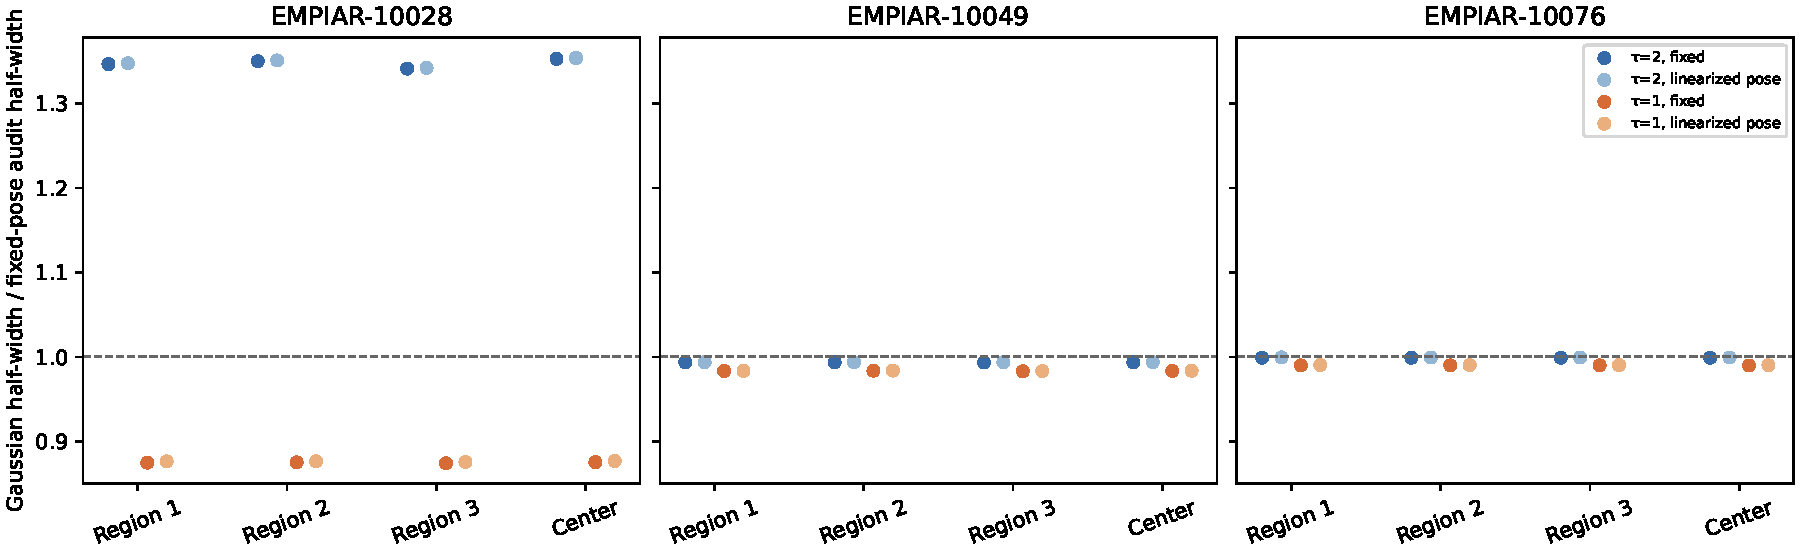
\includegraphics[width=\textwidth]{figures/continuous-gaussian-v2.pdf}
\caption{All twelve locked features and four continuous Gaussian comparisons.
The dashed line denotes the original fixed-pose audit width. Matched prior
scale $\tau=2$ gives near-equal widths on two stacks; its 10028 widths are
34--35\% larger. The half-scale prior is narrower without the same uniform
class implication. Adding the specified first-order Gaussian pose covariance
has little effect here. Every fit converged.}
\label{fig:matchedgaussian}
\end{figure*}
The three complete setup-and-fit runs take 518, 384 and 373 seconds,
respectively, on the authorized Mac under concurrent load. The process peak
resident memory is 6.08 GB; this is a cumulative process high-water mark,
not a fresh per-geometry memory measurement. All relative CG residuals are
at most $9.61\times10^{-11}$. The original rank-1,024 failures are separate
from these 48 successful numerical fits.
}{}
\begin{table}[t]
\centering\small
\caption{Minimum fixed-pose uniform class coverage across four targets, at nominal $1-.05/12=.995833$. Columns separate the prior scale and fixed/linearized covariance weights. These are analytic class minima, not coverage on a selected generator.}
\label{tab:gpclass}
\begin{tabular}{lrrrr}\toprule
Stack & $2$, fixed & $2$, linear & $1$, fixed & $1$, linear \\\midrule
10028 & 0.999930 & 0.999931 & 0.979915 & 0.980143 \\
10049 & 0.995836 & 0.995842 & 0.994882 & 0.994891 \\
10076 & 0.995840 & 0.995851 & 0.995363 & 0.995375 \\
\bottomrule\end{tabular}\end{table}

At prior scale $B/2$, class-worst-case coverage falls below nominal on all
three stacks, although coverage of the selected simulation generators is
favorable. At scale $B$, all 24 class minima exceed .995836. This distinction
prevents treating coverage of benign generators as a uniform class result.

\subsection{Local-pose refitting study}
The calibration seed root is 261001; the test root is 261002. Each is
combined with dataset identifier and replicate index using NumPy's seed
sequence. Calibration contains 128 datasets per geometry; testing has
exactly 200. New alignment noise, inference noise and local initialization
are independently drawn for each replicate. Templates, truth and acquisition
geometry remain fixed. All templates, targets, methods and image controls
within that replicate are paired, not independent observations.

The optimizer uses the frozen ten-iteration Gauss--Newton procedure and its
unchanged step/search constraints. Oracle-template and independent-pilot
fits share the noisy alignment images and initialization. Pose search is
local around near-truth initialization; we do not claim global orientation
discovery. Estimated translations dephase both observation controls and
estimated rotations define a new Fourier Gram. Every interval weight is
recomputed. The affine inference pilot remains the independent pilot even
when the alignment template is oracle truth. Thus the oracle control
isolates reference quality for alignment, not an oracle density estimator.

Fixed-audit weights minimize the sum objective with 100 maximum iterations
and relative-gap target .005. Gaussian fits use relative CG tolerance
$10^{-10}$ and at most 2,000 iterations. Quadrature order is 40 and
preconditioner rank 1,024. Local-Gaussian pose SDs are calibration RMS errors
per coordinate, without removing mean error. These differ from the fixed
$1^\circ$/.5\,\AA\ values in the separate radius-12 comparison.

All nine procedures, both targets, both templates and both image controls
give 72 interval cells per replicate. The first five procedures retain raw
and no-data-selected results; all four Gaussian procedures are reported
raw. Selection compares widths using the fitted design, not the inference
value. When the no-data interval wins, both center and width switch to the
pilot/class interval. It can obtain coverage with no sign information, so
fallback rate and raw outcomes must accompany selected coverage.

Every attempted replicate writes a JSON and arrays, including partial
arrays and exception text on failure. Failed trials remain in the planned
denominator of 200. A completed replicate must contain all 72 unique cells.
Summaries require all 200 attempts and recheck hashes of every JSON, array
and calibration input. Exact binomial 95\% intervals quantify Monte Carlo
uncertainty separately for each procedure; they are not simultaneous
confidence bands over all displayed comparisons. Width summaries use the
available outcomes and report their count. Paired image-control discordance
counts and center differences are retained. Empirical cross-particle
correlations and mean errors are unconditional diagnostics, not tests that
establish conditional-on-design centering.
All 600 datasets and 12,000 solves complete. The total recorded test runtime is 19,584 seconds; peak resident memory is below .681 GB per process. All 216 raw/selected coverage fractions are one. The selected pose intervals use no inference information, so their perfect observed coverage is not an informativeness result. All paired coverage discordance counts are zero. The no-data reference is itself conditional on the supplied pilot-centered class; relative width is not biological resolution.

The final pose errors are substantially larger than the near-truth initialization: rotation RMS medians span 11.990--18.481 degrees and shift medians 6.617--9.282\,\AA. Calibration radii are determined by these same poor local-fitting dynamics. The post-outcome arithmetic remainder decomposition retains all 2,400 template/target fits and does not change an interval or scientific parameter. Minimum and maximum nonlinear-remainder fractions of the raw mixed-zero width are .993056 and .995307. The detailed records include all pose errors, unconditional dependence diagnostics, centers, absolute widths, widths relative to estimates and paired differences.
All 216 detailed coverage, fallback and sign-exclusion rows and both heat maps remain in the machine-readable release. Since every coverage entry is one and every pose fallback entry is one, the compact main table reports their common outcome without repeating three pages of identical entries.
\begin{table*}[t]
\centering\footnotesize
\caption{Post hoc audit-weight diagnostics. Each pair is same-image / independent-image; every cell has 200 paired trials. RMSE is divided by the fixed pilot absolute error. The complete release includes all five distinct estimators, all radius choices, and individual Monte Carlo intervals.}
\label{tab:refittingbias}
\begin{tabular}{lllrrr}\toprule
Stack & Pose control & Target & Mean error / SD & Noise-only coverage & RMSE / pilot error \\\midrule
10028 & True poses & center & -0.367 / -0.400 & 0.920 / 0.925 & 0.061 / 0.062 \\
10028 & True poses & contrast & -0.099 / -0.139 & 0.965 / 0.965 & 0.276 / 0.311 \\
10028 & Oracle template & center & -0.258 / -0.539 & 0.925 / 0.895 & 0.056 / 0.069 \\
10028 & Oracle template & contrast & -0.156 / 0.137 & 0.960 / 0.935 & 0.265 / 0.297 \\
10028 & Pilot template & center & -1.177 / -1.266 & 0.815 / 0.750 & 0.085 / 0.092 \\
10028 & Pilot template & contrast & 0.217 / 0.239 & 0.965 / 0.940 & 0.299 / 0.325 \\
10049 & True poses & center & 0.081 / 0.070 & 0.930 / 0.980 & 1.432 / 1.391 \\
10049 & True poses & contrast & 0.198 / 0.194 & 0.930 / 0.955 & 1.029 / 0.999 \\
10049 & Oracle template & center & 0.737 / -0.295 & 0.900 / 0.925 & 1.590 / 1.478 \\
10049 & Oracle template & contrast & -0.128 / 0.656 & 0.950 / 0.895 & 0.757 / 1.018 \\
10049 & Pilot template & center & 0.638 / -0.557 & 0.905 / 0.925 & 1.600 / 1.594 \\
10049 & Pilot template & contrast & 1.007 / 1.349 & 0.860 / 0.720 & 1.127 / 1.350 \\
10076 & True poses & center & -0.282 / -0.173 & 0.920 / 0.960 & 0.343 / 0.314 \\
10076 & True poses & contrast & -0.068 / -0.161 & 0.955 / 0.925 & 0.758 / 0.872 \\
10076 & Oracle template & center & 0.363 / -0.384 & 0.955 / 0.915 & 0.317 / 0.330 \\
10076 & Oracle template & contrast & 0.165 / -0.024 & 0.950 / 0.945 & 0.689 / 0.797 \\
10076 & Pilot template & center & 0.941 / -0.325 & 0.860 / 0.935 & 0.433 / 0.332 \\
10076 & Pilot template & contrast & -0.162 / 0.081 & 0.965 / 0.950 & 0.718 / 0.792 \\
\bottomrule\end{tabular}
\end{table*}


\subsection{Experimental breakdown analysis}
For each fixed estimator, the stored pilot, density-radius coefficient,
pose remainder and noise scale determine a width as $B$ or measurement SD
is varied. The reporting script reconstructs the stored $B=2$ result to
$10^{-9}$ tolerance before solving where the interval first contains zero.
It reports all 96 feature/pose/calibration combinations; it does not refit
weights at each radius. A breakdown of zero means the feature already
fails sign exclusion at zero radius or noise. It is not evidence that the
true density radius is zero.

At one degree, every retained fixed-weight bias bound already exceeds the
observed center at zero measurement SD. At fixed poses, centered-calibration
10028 breakdowns range from 2.877 to 4.868. These sensitivities measure how
far an assumed input can move before a reported conclusion changes; they
do not estimate that input or validate the common-noise law. The inference
centers were known before this analysis. All raw/selected widths,
no-data-fallback flags and registered-reference disagreements remain saved.
\IfFileExists{tables/breakdown-radii.tex}{\begin{table*}[p]
\centering\small
\caption{Density-radius breakdowns for every locked feature and both experimental noise calibrations. Each pair is raw/centered calibration. Zero means sign exclusion already fails at $B=0$; the declared radius is $B=2$. These are fixed-weight sensitivity thresholds, not estimates of the true radius. Every one-degree noise-scale breakdown is zero. Full half-width/center ratios, noise thresholds and fallback flags are retained in the all-case CSV.}
\begin{tabular}{llrrrr}
\toprule
Stack & Feature & Fixed poses & Shifts only & One degree & Two degrees \\
\midrule
10028 & Region 1 & 3.447/4.832 & 0.516/0.757 & 0.000/0.000 & 0.000/0.000 \\
10028 & Region 2 & 3.444/4.868 & 0.542/0.807 & 0.000/0.000 & 0.000/0.000 \\
10028 & Region 3 & 1.595/2.877 & 0.187/0.395 & 0.000/0.000 & 0.000/0.000 \\
10028 & Center & 1.612/3.055 & 0.193/0.457 & 0.000/0.000 & 0.000/0.000 \\
\addlinespace
10049 & Region 1 & 0.000/153.172 & 0.000/3.401 & 0.000/0.000 & 0.000/0.000 \\
10049 & Region 2 & 0.000/0.000 & 0.000/0.000 & 0.000/0.000 & 0.000/0.000 \\
10049 & Region 3 & 0.000/0.000 & 0.000/0.000 & 0.000/0.000 & 0.000/0.000 \\
10049 & Center & 0.000/133.654 & 0.000/2.854 & 0.000/0.000 & 0.000/0.000 \\
\addlinespace
10076 & Region 1 & 119.076/186.381 & 7.143/11.239 & 0.000/0.054 & 0.000/0.000 \\
10076 & Region 2 & 68.808/126.048 & 4.158/7.692 & 0.000/0.000 & 0.000/0.000 \\
10076 & Region 3 & 111.064/178.140 & 6.626/10.713 & 0.000/0.016 & 0.000/0.000 \\
10076 & Center & 89.151/161.521 & 5.332/9.752 & 0.000/0.000 & 0.000/0.000 \\
\addlinespace
\bottomrule
\end{tabular}
\end{table*}
}{}

\subsection{Reconstruction baselines and FSC interpretation}
Stock cryoDRGN 4.3.1 homogeneous training uses supplied consensus poses,
three hidden layers of width 256 and batch size eight, separately on both
exposure-group halves of each stack. These are actual neural fits, not
backprojection, but are not ab initio CryoDRGN-AI or uncertainty inference.
Gaussian and voxel ridge fits use those same halves. Held-out image scoring
uses identical particles, 1,410 Fourier pairs per image inside radius 30
of a 64-pixel grid, and the same window/background normalization. Stock
neural training uses its radius-32 loss and per-half global scale, so the
training objectives differ. Tuning-group prediction error selects epochs
60, 50 and 100; two are final available checkpoints and undertraining
remains possible. The development stopping budgets are not preregistered
convergence criteria.
\begin{table*}[t]
\centering
\caption{Frozen additional-exposure prediction: 4,096 particles per dataset from 115, 71 and 185 source groups absent from development. Models and cohort were locked before image access. Lower normalized prediction MSE is better. Supplied consensus poses/CTFs remain conditional; this does not measure unknown density coverage.}
\label{tab:freshprediction}
\begin{tabular}{lrrr}\toprule
EMPIAR & Gaussian & Voxel & Neural \\\midrule
10028 & 0.835319 & 0.841379 & 0.829369 \\
10049 & 0.931579 & 0.932359 & 0.930739 \\
10076 & 0.874799 & 0.879078 & 0.868657 \\
\bottomrule\end{tabular}
\medskip

\begin{tabular}{llrl}\toprule
EMPIAR & Comparator minus neural & NMSE difference & Adjusted percentile interval \\\midrule
10028 & Gaussian & 0.005950 & [0.004995, 0.006932] \\
10028 & Voxel & 0.012011 & [0.010695, 0.013356] \\
10049 & Gaussian & 0.000840 & [0.000659, 0.001023] \\
10049 & Voxel & 0.001620 & [0.001366, 0.001875] \\
10076 & Gaussian & 0.006143 & [0.005686, 0.006593] \\
10076 & Voxel & 0.010421 & [0.009792, 0.011038] \\
\bottomrule\end{tabular}
\par\small{All six prespecified paired differences are shown. Intervals use 10,000 whole-exposure bootstrap resamples and a Bonferroni adjustment for six contrasts (99.1667\% marginal percentile intervals). This is a bootstrap approximation, not a finite-sample coverage theorem. No model selection uses these outcomes.}
\end{table*}


RELION 5.0.1 learns poses on all three stacks using a common prescribed
initialization/refinement protocol, with exposure-half labels verified.
Wall-limited initial attempts and separately declared continuations remain
available. No checkpoint is chosen by reference FSC. Native half FSC is
computed before map registration, unmasked, with the coupled low-frequency
region displayed: RELION joins halves below $1/40$\,\AA$^{-1}$.
Cross-method and external-reference FSC use the fixed pilot-only frame/hand
transform, retaining interpolation and registration limits. All native and
registered curves are provided, including poor agreement.

\begin{figure*}[t]
\centering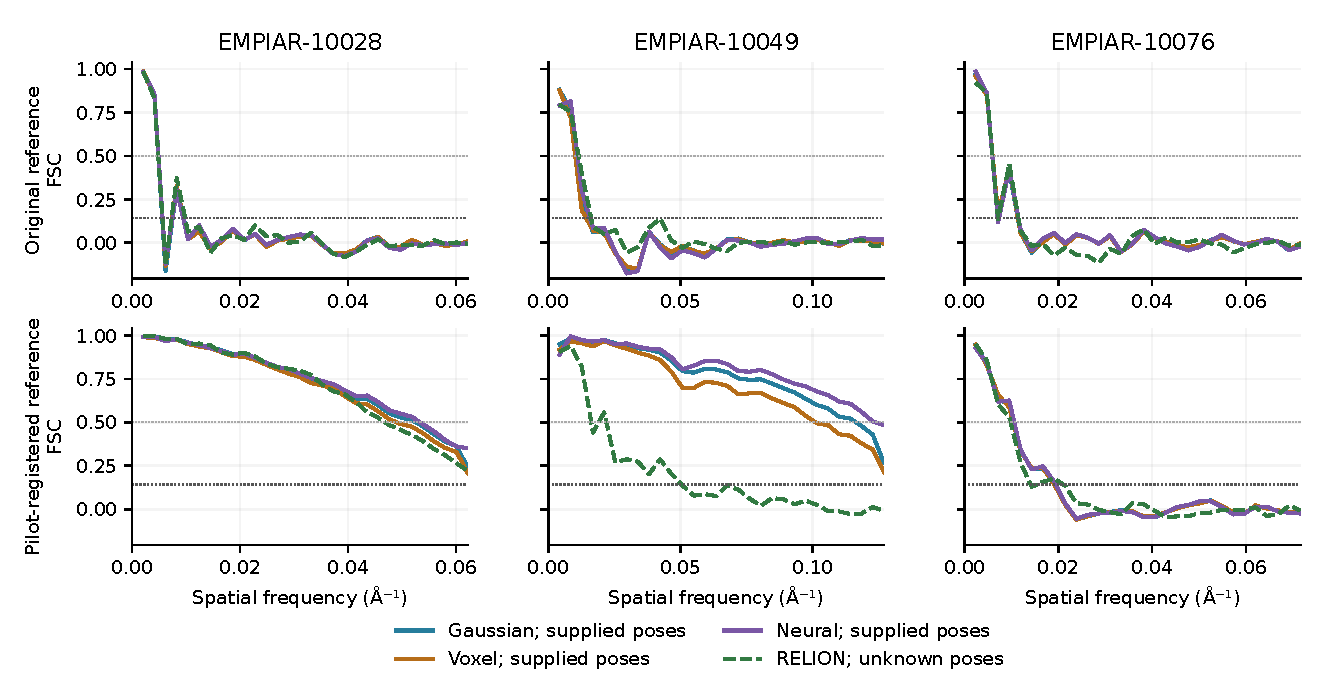
\includegraphics[width=\textwidth]{figures/registered-reconstruction-fsc.pdf}
\caption{All twelve reconstruction method/stack comparisons against original
and pilot-registered references; dotted lines mark FSC 0.5 and 0.143.
Gaussian, voxel and neural fits use supplied poses; RELION estimates poses.
The old pilot alone determines registration. Agreement includes preprocessing,
interpolation and frame dependence. Censored crossings are not measured
resolutions. The 10076 Class A reference is not truth for its heterogeneous
consensus, and none of these curves measures interval coverage.}
\label{fig:registeredfsc}
\end{figure*}

For 10049, native FSC crosses .5 at 22.73\,\AA\ and .143 at
18.95\,\AA. For 10076 these crossings are 24.73 and 15.92\,\AA.
The registered-reference mean FSCs are .702, .202 and .122 for 10028,
10049 and 10076. Mean FSC is a descriptive average over the recorded shells,
not a resolution measure. The heterogeneous third stack and state-specific
reference limit interpretation. Half-map agreement above a threshold
through the sampled band is reported as censored at that limit, not an
observed threshold crossing. Algorithmic convergence also does not establish
structural accuracy.

Original-code CryoLike likelihood scoring and held-out prediction provide
additional image-fit context. A likelihood or FSC is not a confidence
interval for the unknown true feature; we do not use those methods as if
they promised such coverage. Conversely, weak reconstruction agreement is
not hidden by reporting only an uncertainty diagnostic.
Figures~\ref{fig:slices10028}--\ref{fig:slices10076} show every method
in the same three central planes, with display normalization stated explicitly.
\begin{figure*}[p]
\centering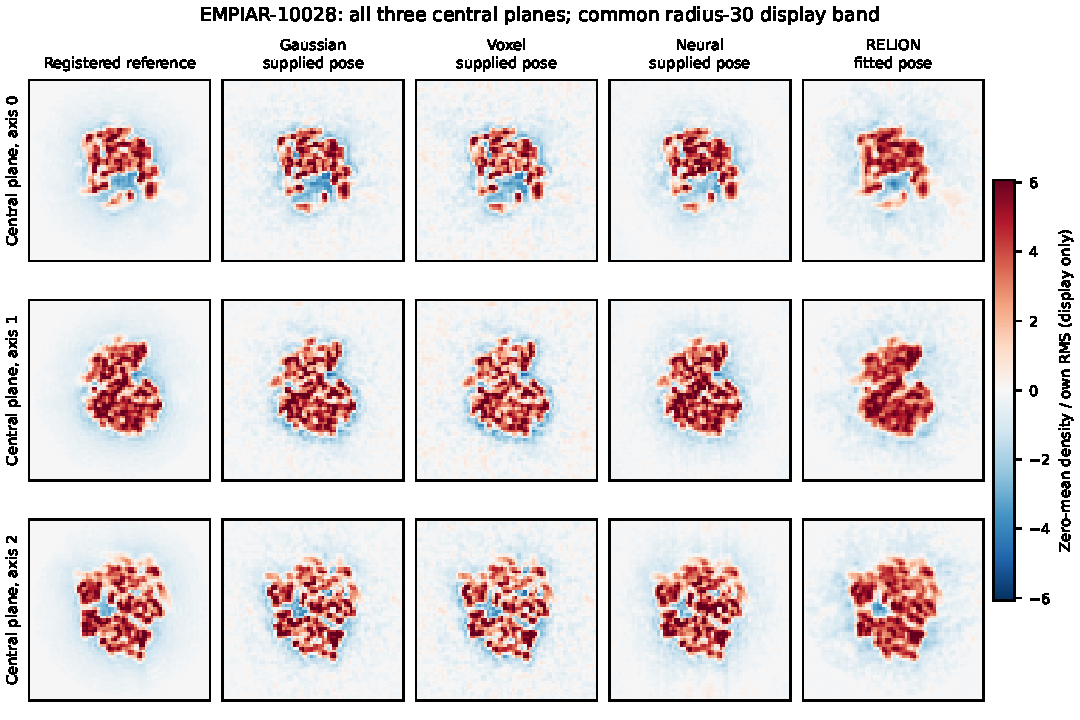
\includegraphics[width=\textwidth]{figures/reconstruction-slices-10028.pdf}
\caption{EMPIAR-10028: all three central planes of the registered reference and four existing reconstructions. Each square spans 482.4\,\AA. The display removes DC, retains a common radius-30 Fourier band, and divides each map by its own volumetric RMS; a pooled 99.5th-percentile absolute value fixes the common symmetric color range. This display normalization hides amplitude differences and is not used for FSC or intervals. Views are fixed array planes, not selected for agreement. Gaussian, voxel and neural estimates average the locked halves; RELION uses its previously evaluated map. Registration is pilot-derived. The 10076 reference represents Class A, not the heterogeneous consensus.}
\label{fig:slices10028}
\end{figure*}
\begin{figure*}[p]
\centering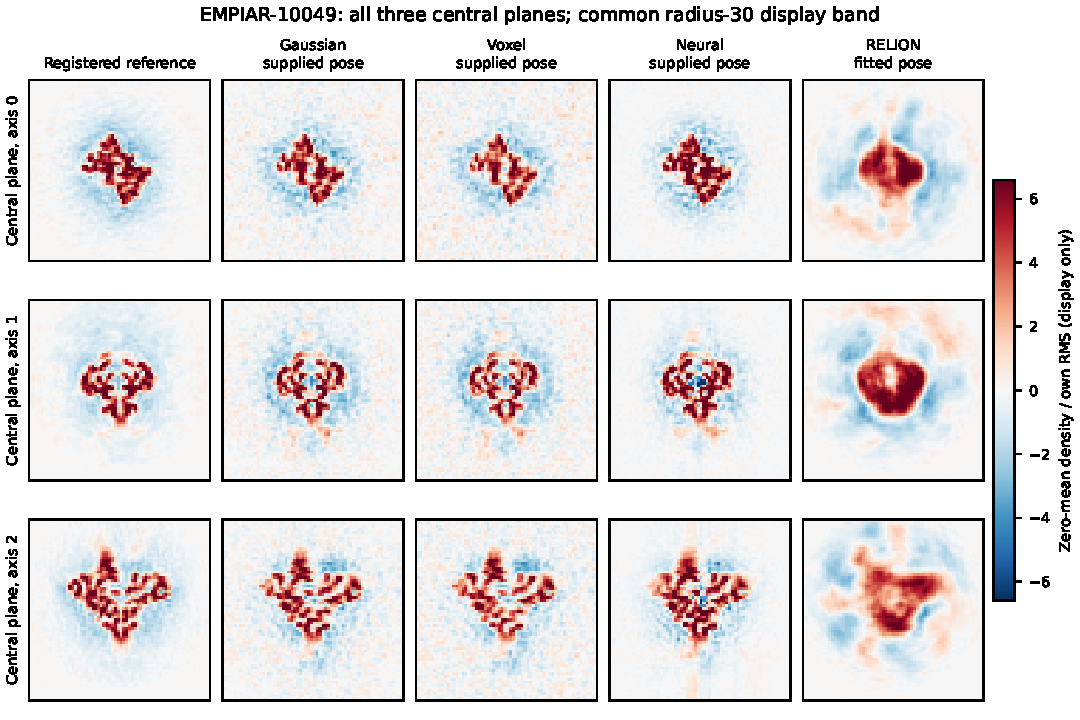
\includegraphics[width=\textwidth]{figures/reconstruction-slices-10049.pdf}
\caption{EMPIAR-10049: all three central planes of the registered reference and four existing reconstructions. Each square spans 236.16\,\AA. The display removes DC, retains a common radius-30 Fourier band, and divides each map by its own volumetric RMS; a pooled 99.5th-percentile absolute value fixes the common symmetric color range. This display normalization hides amplitude differences and is not used for FSC or intervals. Views are fixed array planes, not selected for agreement. Gaussian, voxel and neural estimates average the locked halves; RELION uses its previously evaluated map. Registration is pilot-derived. The 10076 reference represents Class A, not the heterogeneous consensus.}
\label{fig:slices10049}
\end{figure*}
\begin{figure*}[p]
\centering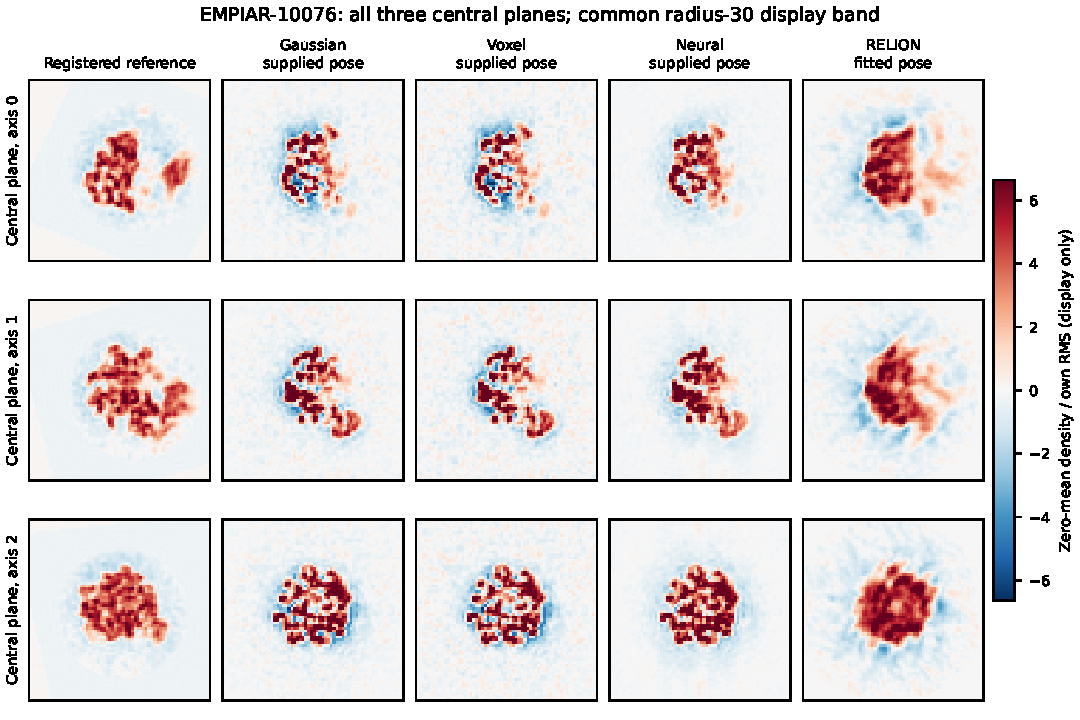
\includegraphics[width=\textwidth]{figures/reconstruction-slices-10076.pdf}
\caption{EMPIAR-10076: all three central planes of the registered reference and four existing reconstructions. Each square spans 419.2\,\AA. The display removes DC, retains a common radius-30 Fourier band, and divides each map by its own volumetric RMS; a pooled 99.5th-percentile absolute value fixes the common symmetric color range. This display normalization hides amplitude differences and is not used for FSC or intervals. Views are fixed array planes, not selected for agreement. Gaussian, voxel and neural estimates average the locked halves; RELION uses its previously evaluated map. Registration is pilot-derived. The 10076 reference represents Class A, not the heterogeneous consensus.}
\label{fig:slices10076}
\end{figure*}


\subsection{Raw-movie feasibility and remaining dependence}
A separately declared acquisition pilot downloaded one EMPIAR-10028 movie,
\texttt{Micrographs\_part2/004\_movie.mrcs}, with 16 frames of
$4096\times4096$ float32 pixels. The source-group mapping is supported by
archive counts, acquisition date and nearby coordinates, but the deposited
autopicks differ from final recentered coordinates. It is not labeled a
fully verified new confirmatory cohort. Its completed analysis is restricted
to all-frame acquisition statistics, a fixed patch grid, frame-difference
spectra/correlations and unaligned odd/even sums. Differences can contain
motion, dose signal and detector effects; they are not automatically pure
noise or proof of frame independence. No density intervals result from this
pilot. Any subsequent motion, picking, CTF or alignment pipeline requires
its own declared processing graph and cannot claim independent inference
noise while silently reusing full-movie-derived quantities.

All sixteen frames, 512 fixed patch differences and 1,792 cross-pair
correlations were retained. Median horizontal and vertical neighbor
correlations are .657 and .658; the 5th--95th percentiles of disjoint
difference correlation are $-.00780$ to $.00866$. Frame means span
2052.53--2060.28 in deposited pixel units. The difference fields are spatially
correlated; these statistics do not separate detector noise from residual
signal. Small temporal correlations do not establish independence or a
transferable covariance.
The interrupted download and verified byte-range recovery are preserved;
they did not change the predeclared movie or diagnostics.
\begin{table*}[t]
\centering\small
\caption{Predeclared acquisition diagnostics from one raw 10028 movie. Difference statistics use every one of 512 patch/pair combinations; disjoint-pair correlations use all 1,792 comparisons. Quantiles are descriptive across dependent summaries, not independent-replicate confidence intervals.}
\begin{tabular}{lrrrrr}
\toprule
Statistic & Minimum & 5th percentile & Median & 95th percentile & Maximum \\
\midrule
Difference SD & 341.7 & 351.2 & 357.7 & 370.3 & 402.5 \\
Horizontal neighbor correlation & 0.6455 & 0.6496 & 0.6569 & 0.6641 & 0.6844 \\
Vertical neighbor correlation & 0.6463 & 0.6522 & 0.6583 & 0.6662 & 0.6862 \\
Disjoint-difference correlation & -0.01856 & -0.007798 & 0.0006576 & 0.008661 & 0.01639 \\
\bottomrule
\end{tabular}
\end{table*}

